% Two charts E_1, E_2 of a 1-manifold, glued over the interval [0,2] in R,
% with linear transition maps phi_1, phi_2.
% Source: book/tex/riemann-surface/complex-structure.tex (§ Transition maps).
\documentclass[border=2mm]{standalone}
\usepackage{tikz}
\usepackage{amssymb}
\usetikzlibrary{calc}
\begin{document}
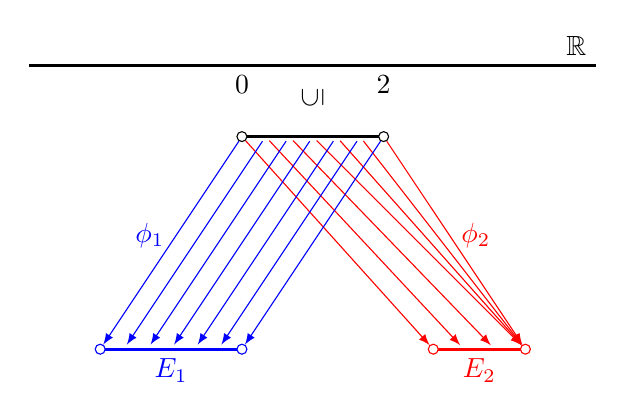
\begin{tikzpicture}[>=latex, scale=0.9]
  \draw[very thick] (0,5)--(8,5);
  \node[above left] at (8,5) {$\mathbb{R}$};
  \draw[very thick] (3,4)--(5,4);
  \draw[fill=white] (3,4) circle(2pt); \draw[fill=white] (5,4) circle(2pt);
  \node[rotate=90] at (4,4.55) {$\subseteq$};
  \node[below] at (3,5) {$0$}; \node[below] at (5,5) {$2$};
  \draw[blue, very thick] (1,1)--(3,1);
  \draw[blue,fill=white] (1,1) circle(2pt); \draw[blue,fill=white] (3,1) circle(2pt);
  \node[blue,below] at (2,1) {$E_1$};
  \draw[red, very thick] (5.7,1)--(7,1);
  \draw[red,fill=white] (5.7,1) circle(2pt); \draw[red,fill=white] (7,1) circle(2pt);
  \node[red,below] at (6.35,1) {$E_2$};
  \foreach \i in {0,...,6}{
    \draw[blue,->,shorten >=2pt,shorten <=2pt] ($(3,4)+\i*(0.3333,0)$)--($(1,1)+\i*(0.3333,0)$);
    \pgfmathtruncatemacro\j{min(\i,3)}
    \draw[red,->,shorten >=2pt,shorten <=2pt] ($(3,4)+\i*(0.3333,0)$)--($(5.7,1)+\j*(0.4333,0)$);
  }
  \node[blue] at (1.7,2.6) {$\phi_1$};
  \node[red] at (6.3,2.6) {$\phi_2$};
\end{tikzpicture}
\end{document}
